
\documentclass[aspectratio=169]{beamer}

\usetheme{durham}

%========================================================
% Durham Beamer Theme – Teaching-Focused Demo
%========================================================

\title{The Durham Beamer Theme}
\subtitle{A Content-First Academic Presentation System}
\author{Beamer Atelier}
\institute{Design Studio Executive}
% Keep the demo date aligned with the package release date.
\date{23 February 2026}

\begin{document}

\maketitle
\DurhamOutline

%========================================================
\section{Motivation}
%========================================================
\begin{frame}{Beamer Presentation Ecosystem}
Beamer already has a rich and well-established ecosystem in academia:
\begin{itemize}
  \item a wide range of themes,
  \item a strong structural model for presentations,
  \item excellent support for mathematics and technical content.
\end{itemize}

\vspace{0.8em}
It remains the default tool for many lecturers and researchers.
\end{frame}

\begin{frame}{What was missing in practice}
Despite this richness, sustained teaching use revealed recurring issues:
\begin{itemize}
  \item themes optimised for \emph{slides}, not for \emph{lectures},
  \item navigation elements that compete with content rather than support it,
  \item visual noise accumulating over long teaching sessions,
  \item limited support for pacing, time awareness, and audience orientation.
\end{itemize}

\vspace{0.6em}
Most importantly, accessibility considerations were often absent or implicit.
\end{frame}
\subsection{Teaching-Centric}
\begin{frame}{Teaching as the primary use case}
In teaching contexts, presentations function differently:
\begin{itemize}
  \item lectures unfold over time rather than as standalone slides,
  \item students benefit from a sense of structure and progress,
  \item visual consistency reduces cognitive load,
  \item accessibility is not optional, but integral to inclusive teaching.
\end{itemize}

\vspace{0.6em}
This project began with the question:  
\emph{What would Beamer look like if it were designed first and foremost for teaching?}
\end{frame}

%========================================================
\section{Development}
\subsection{Design Principles}
%========================================================

\begin{frame}{Development philosophy}
The Durham theme was developed from scratch, guided by three principles:
\begin{itemize}
  \item content should dominate the slide, not decoration,
  \item navigation should support orientation without distraction,
  \item visual decisions should scale across long lecture sequences.
\end{itemize}

\vspace{0.6em}
Rather than extending an existing theme, each element was reconsidered independently.
\end{frame}

\begin{frame}{Universal Design for Learning as a motivator}
A key influence was the idea of \textbf{Universal Design for Learning (UDL)}:
\begin{itemize}
  \item provide multiple means of representation,
  \item reduce unnecessary barriers to engagement,
  \item allow flexibility in how material is presented and consumed.
\end{itemize}

\vspace{0.6em}
The theme aims to give lecturers control over presentation modes without fragmenting workflows.
\end{frame}

\begin{frame}{From experience to design}
Design choices were informed by:
\begin{itemize}
  \item repeated use in undergraduate and postgraduate lectures,
  \item long sessions with dense quantitative material,
  \item the need to balance structure with visual calm.
\end{itemize}

\vspace{0.6em}
The result is not stylistic novelty, but a system shaped by real teaching constraints.
\end{frame}

%========================================================
\section{Implementation}
%========================================================

\begin{frame}{Implementation overview}
The Durham theme implements a small number of deliberate structural elements:
\begin{itemize}
  \item sections treated explicitly as lecture chapters,
  \item a headline that indicates the current position in the lecture,
  \item a progress indicator to support pacing and time awareness,
  \item a restrained footline for contextual information.
\end{itemize}
\end{frame}

\begin{frame}{Sections as lecture chapters}
Sections are designed to function as conceptual chapters:
\begin{itemize}
  \item each section opens with a dedicated section page,
  \item students are signposted when the lecture moves to a new topic,
  \item the structure remains visible without interrupting flow.
\end{itemize}

\vspace{0.6em}
This reinforces narrative continuity across long teaching sessions.
\end{frame}

\begin{frame}{Sections as lecture chapters}
Sections are designed to function as conceptual chapters:
\begin{itemize}
  \item each section opens with a dedicated section page,
\end{itemize}
\end{frame}

\begin{frame}{Sections as lecture chapters}
Sections are designed to function as conceptual chapters:
\begin{itemize}
  \item each section opens with a dedicated section page,
  \item students are signposted when the lecture moves to a new topic,
\end{itemize}
\end{frame}

\begin{frame}{Sections as lecture chapters}
Sections are designed to function as conceptual chapters:
\begin{itemize}
  \item each section opens with a dedicated section page,
  \item students are signposted when the lecture moves to a new topic,
  \item the structure remains visible without interrupting flow.
\end{itemize}

\vspace{0.6em}
This reinforces narrative continuity across long teaching sessions.
\end{frame}


\begin{frame}{Headline and orientation}
The headline provides lightweight orientation:
\begin{itemize}
  \item shows the current section in context,
  \item avoids visual competition with slide content,
  \item remains consistent across the lecture.
\end{itemize}

\vspace{0.6em}
The intention is not navigation for navigation’s sake, but reassurance of structure.
\end{frame}

\begin{frame}{Progress and time awareness}
The vertical progress indicator serves two roles:
\begin{itemize}
  \item it gives students a sense of how the lecture is unfolding,
  \item it helps lecturers manage pacing and time allocation.
\end{itemize}

\vspace{0.6em}
Importantly, it remains visually quiet and does not rely on colour alone.
\end{frame}

\begin{frame}{Footline as contextual metadata}
The footline is intentionally minimal:
\begin{itemize}
  \item short title and author for orientation,
  \item no duplication of information already present elsewhere,
  \item can be disabled entirely when distraction-free modes are preferred.
\end{itemize}
\end{frame}

\begin{frame}{Colour palette and institutional feel}
The default colour palette is inspired by Durham University:
\begin{itemize}
  \item chosen to convey a calm institutional aesthetic,
  \item consistent with sustained reading and projection.
\end{itemize}

\vspace{0.6em}
However:
\begin{itemize}
  \item this is \textbf{not} an official university theme,
  \item it does not use any trademarks or protected branding,
  \item documentation explicitly clarifies this distinction.
\end{itemize}
\end{frame}
\subsection{Saving Space}

\begin{frame}{Subsections without visual penalty}
This slide intentionally introduces a subsection to illustrate a design choice.

\medskip
In the Durham theme:
\begin{itemize}
  \item the subsection indicator appears \emph{only when a subsection exists},
  \item no reserved or shaded space is shown otherwise,
  \item vertical space is returned to the content when subsections are absent.
\end{itemize}

\medskip
This avoids persistent visual placeholders and returns scarce vertical space to content when structure is not needed.
\end{frame}


%========================================================
\section{Accessibility}
\subsection{Modes}
%========================================================
\begin{frame}{Accessibility options}
\begin{itemize}
  \item The Durham theme includes optional modes to support:
  \begin{itemize}
    \item high-contrast viewing (colour-vision impairment),
    \item distraction-free reading (cognitive load),
    \item reduced visual fatigue (dark background preference).
  \end{itemize}
  \item All modes are opt-in via theme options (comma-separated).
\end{itemize}

\vspace{0.6em}
\textbf{Usage pattern:}
\begin{itemize}
  \item \texttt{\textbackslash usetheme[<options>]\{durham\}}
\end{itemize}
\end{frame}

\begin{frame}[fragile]{Mode 1: \texttt{accessibility} (high contrast, B\&W)}
\begin{itemize}
  \item Switches the palette to black-and-white (high contrast).
  \item Avoids colour-only cues (better for colour-vision deficiencies).
  \item Keeps the theme structure intact (headline/footline/progress).
\end{itemize}

\vspace{0.8em}
\textbf{Enable:}
\begin{verbatim}
\usetheme[accessibility]{durham}
\end{verbatim}
\end{frame}
\begin{frame}[plain]
\begin{figure}
    \centering
    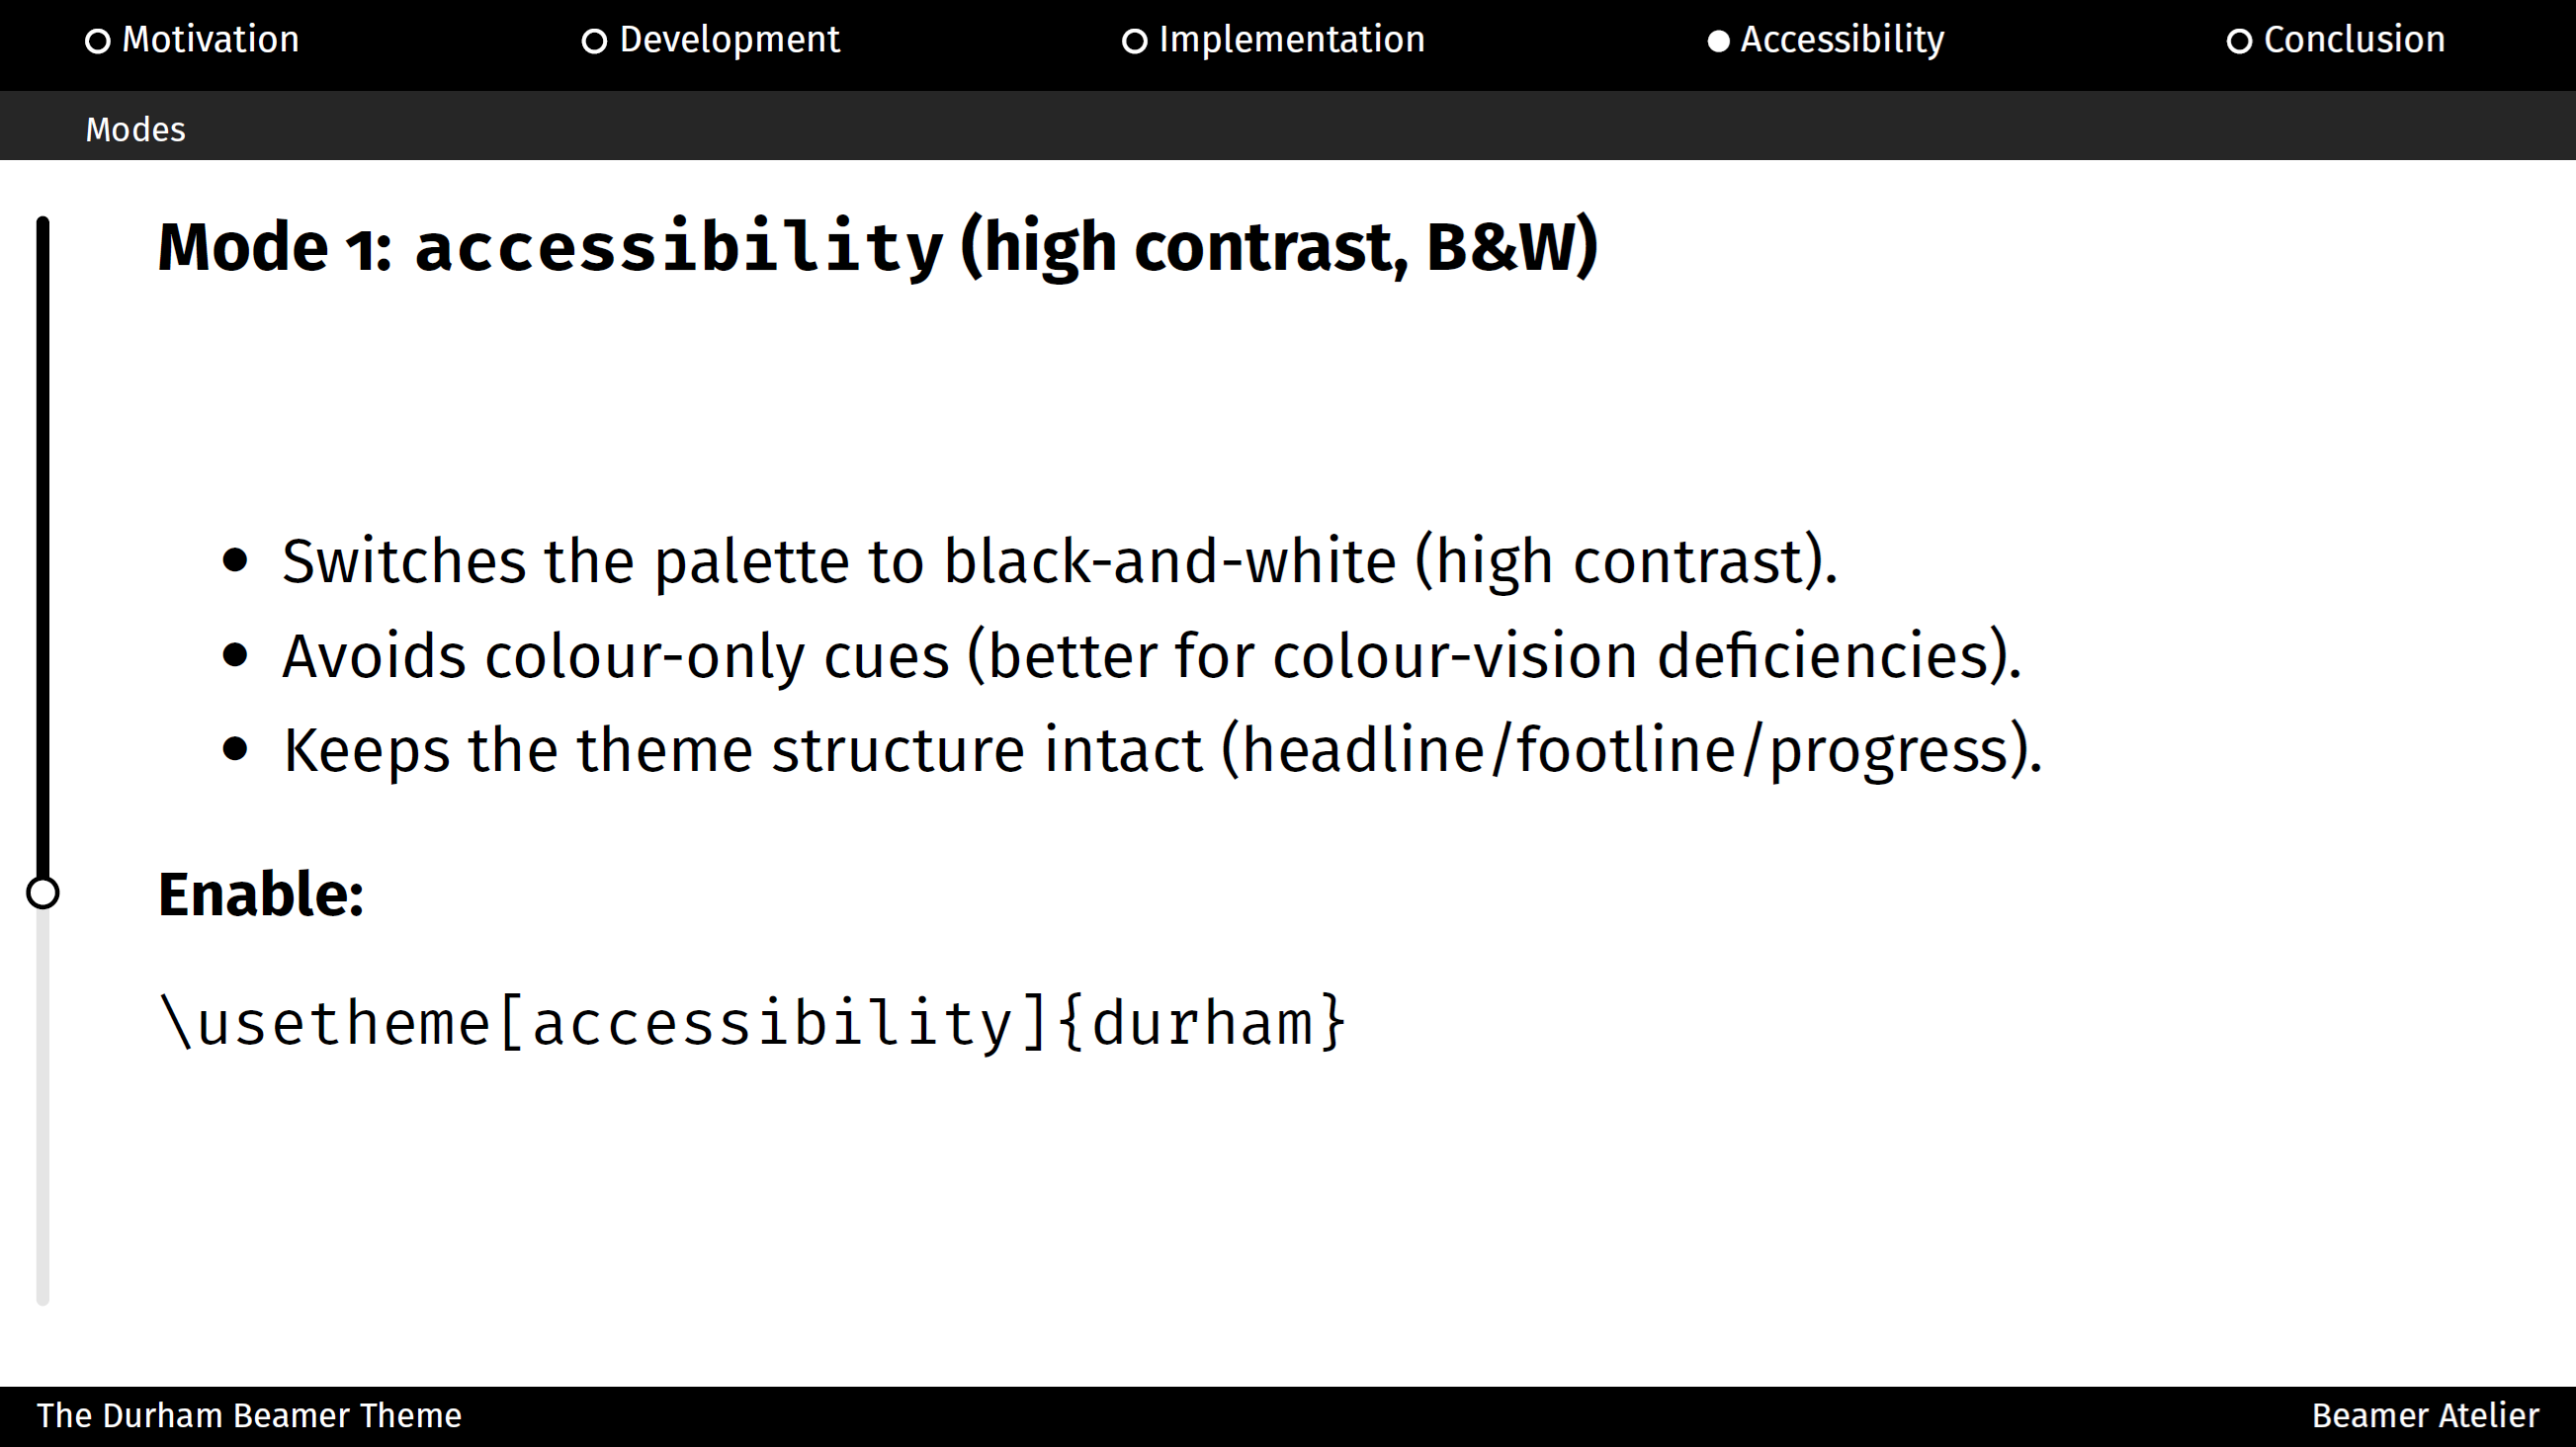
\includegraphics[width=1\linewidth]{accessibility.png}
    \caption{Accessibility Mode}
\end{figure}
\end{frame}


\begin{frame}[fragile]{Mode 2: \texttt{plain} (distraction-free)}
\begin{itemize}
  \item Hides UI elements:
  \begin{itemize}
    \item headline, footline, progress indicators.
  \end{itemize}
  \item Leaves only the slide content for maximum focus.
  \item Useful for dense reading, handouts, or reduced cognitive load.
\end{itemize}

\vspace{0.8em}
\textbf{Enable:}
\begin{verbatim}
\usetheme[plain]{durham}
\end{verbatim}
\end{frame}

\begin{frame}[plain]
\begin{figure}
        \centering
        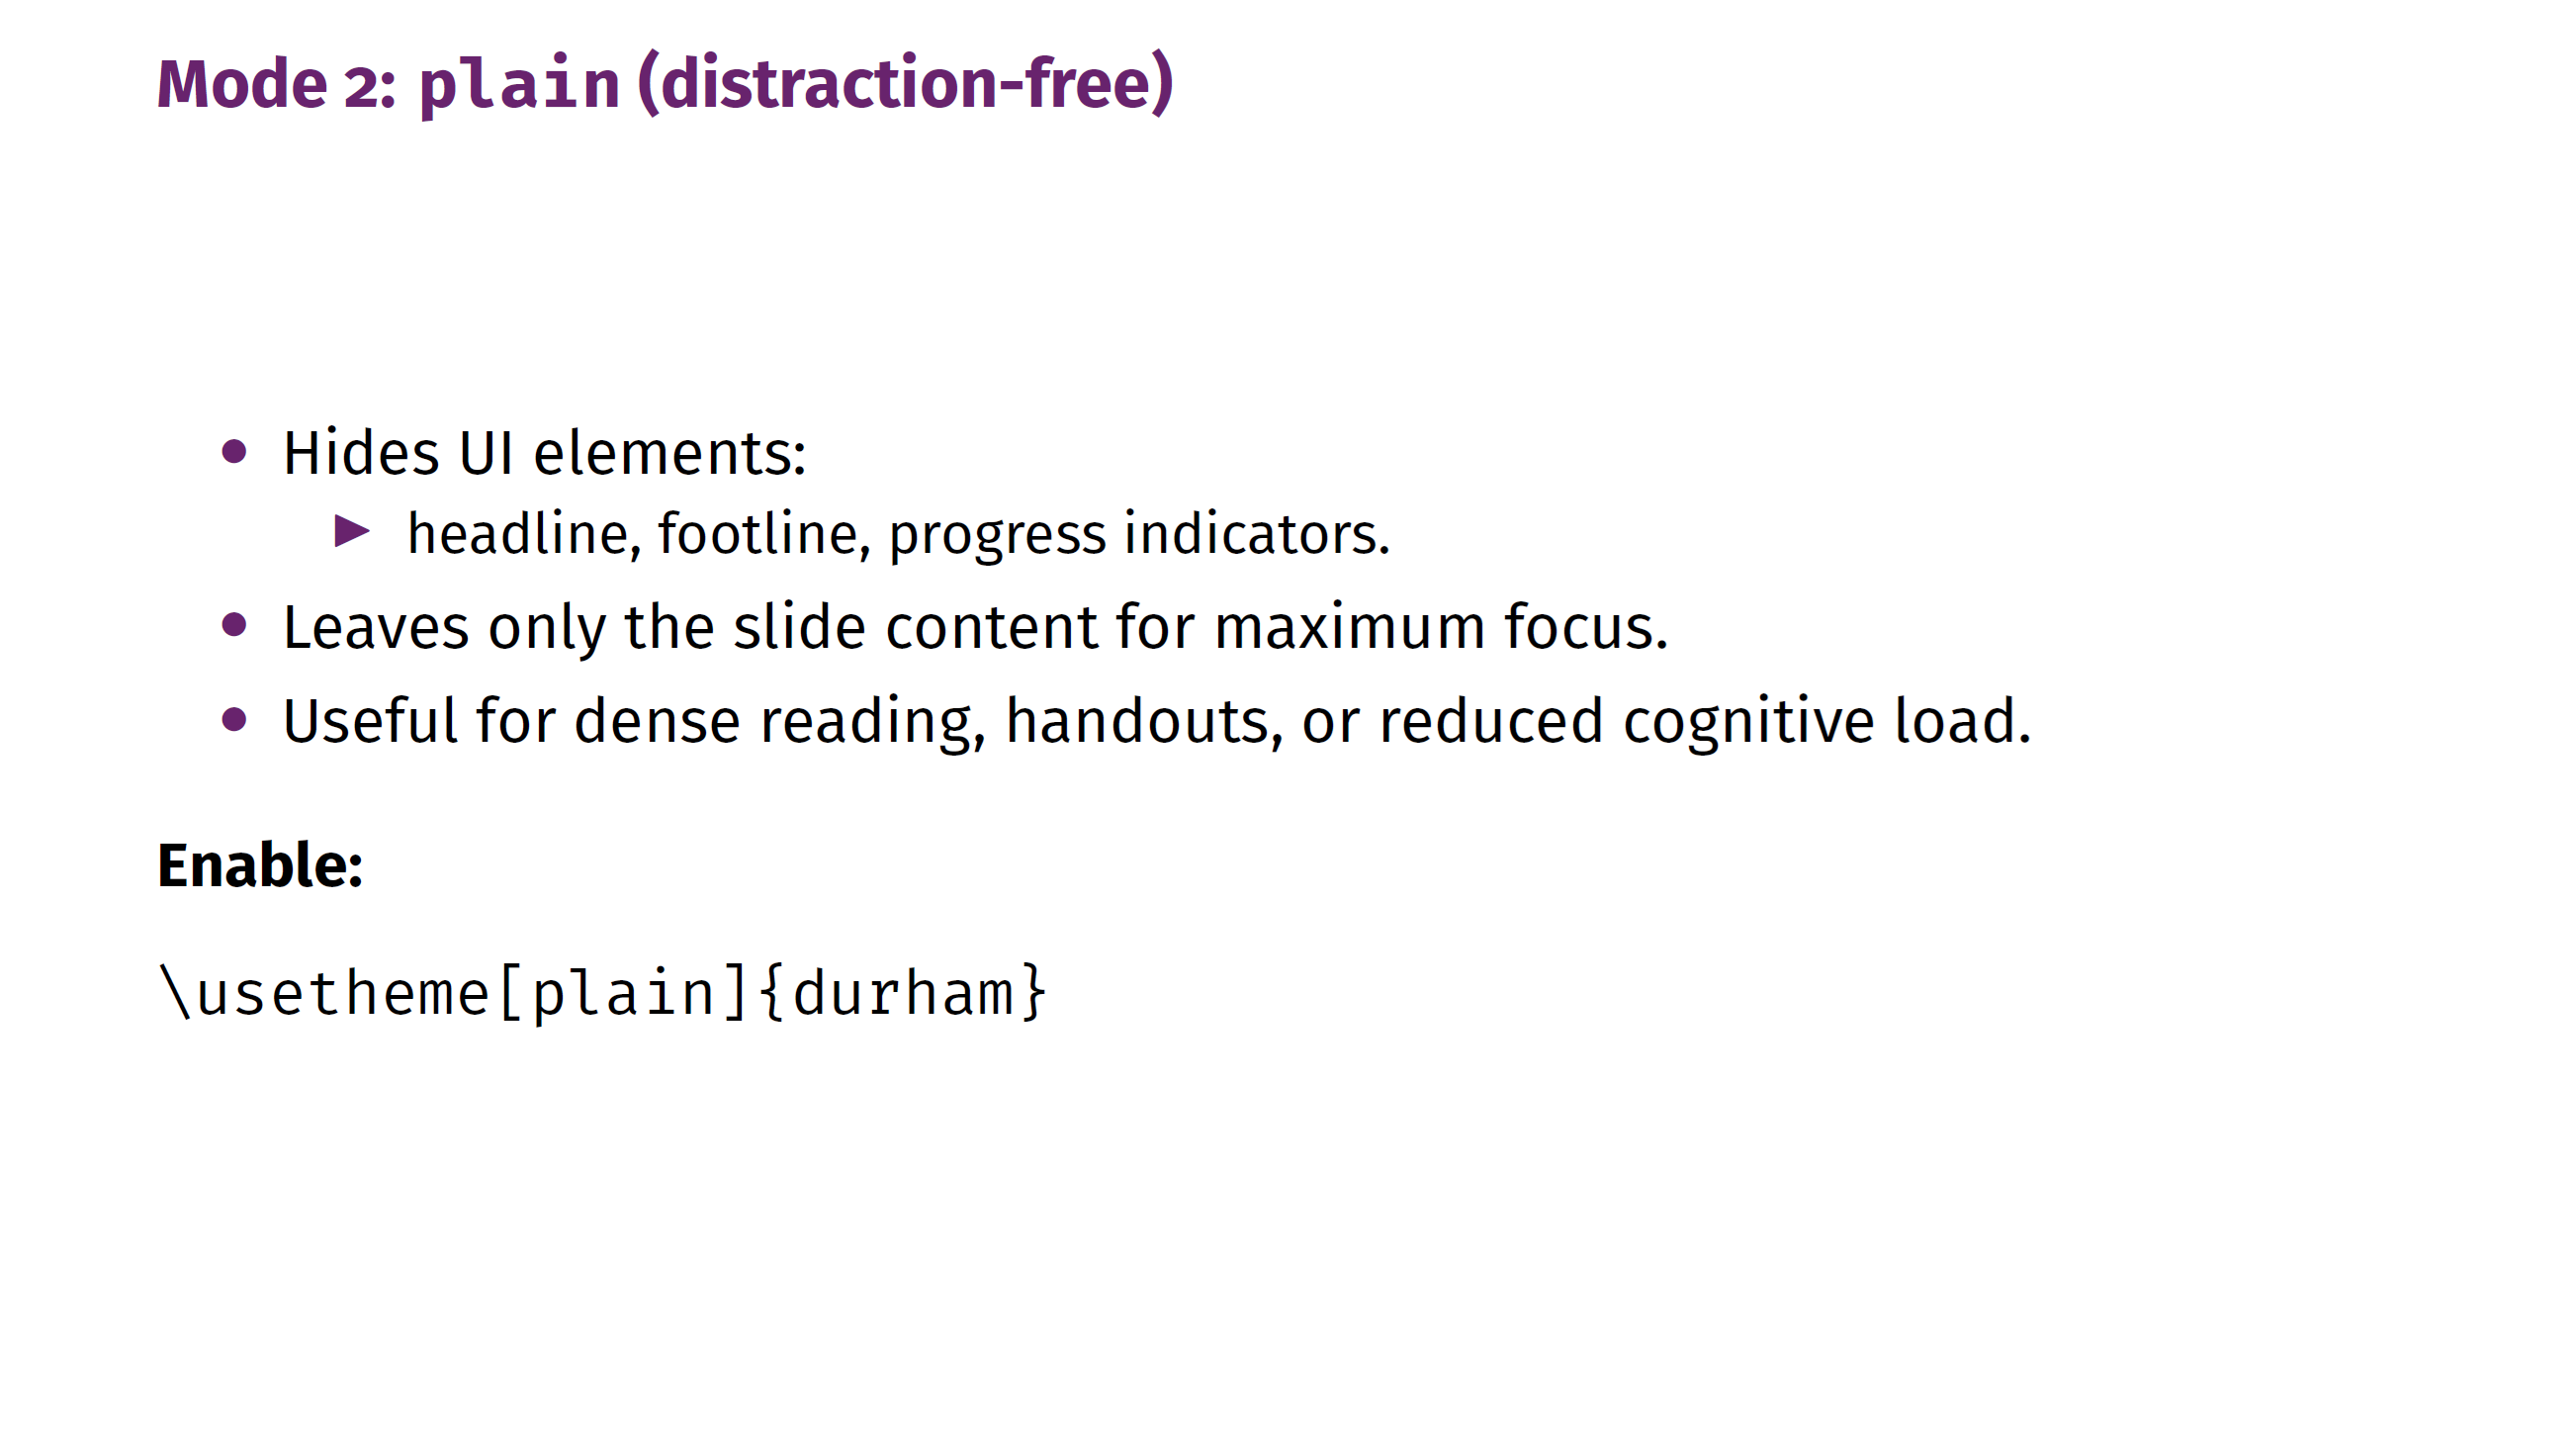
\includegraphics[width=1\linewidth]{plain.png}
        \caption{Plain Mode}
\end{figure}
    
\end{frame}

\begin{frame}[fragile]{Mode 3: \texttt{plain,accessibility} (minimal + B\&W)}
\begin{itemize}
  \item Combines:
  \begin{itemize}
    \item \texttt{plain} (removes UI elements),
    \item \texttt{accessibility} (black text on white background).
  \end{itemize}
  \item A clean reading mode with high-contrast text.
\end{itemize}

\vspace{0.8em}
\textbf{Enable:}
\begin{verbatim}
\usetheme[plain,accessibility]{durham}
\end{verbatim}
\end{frame}

\begin{frame}[plain]
\begin{figure}
    \centering
    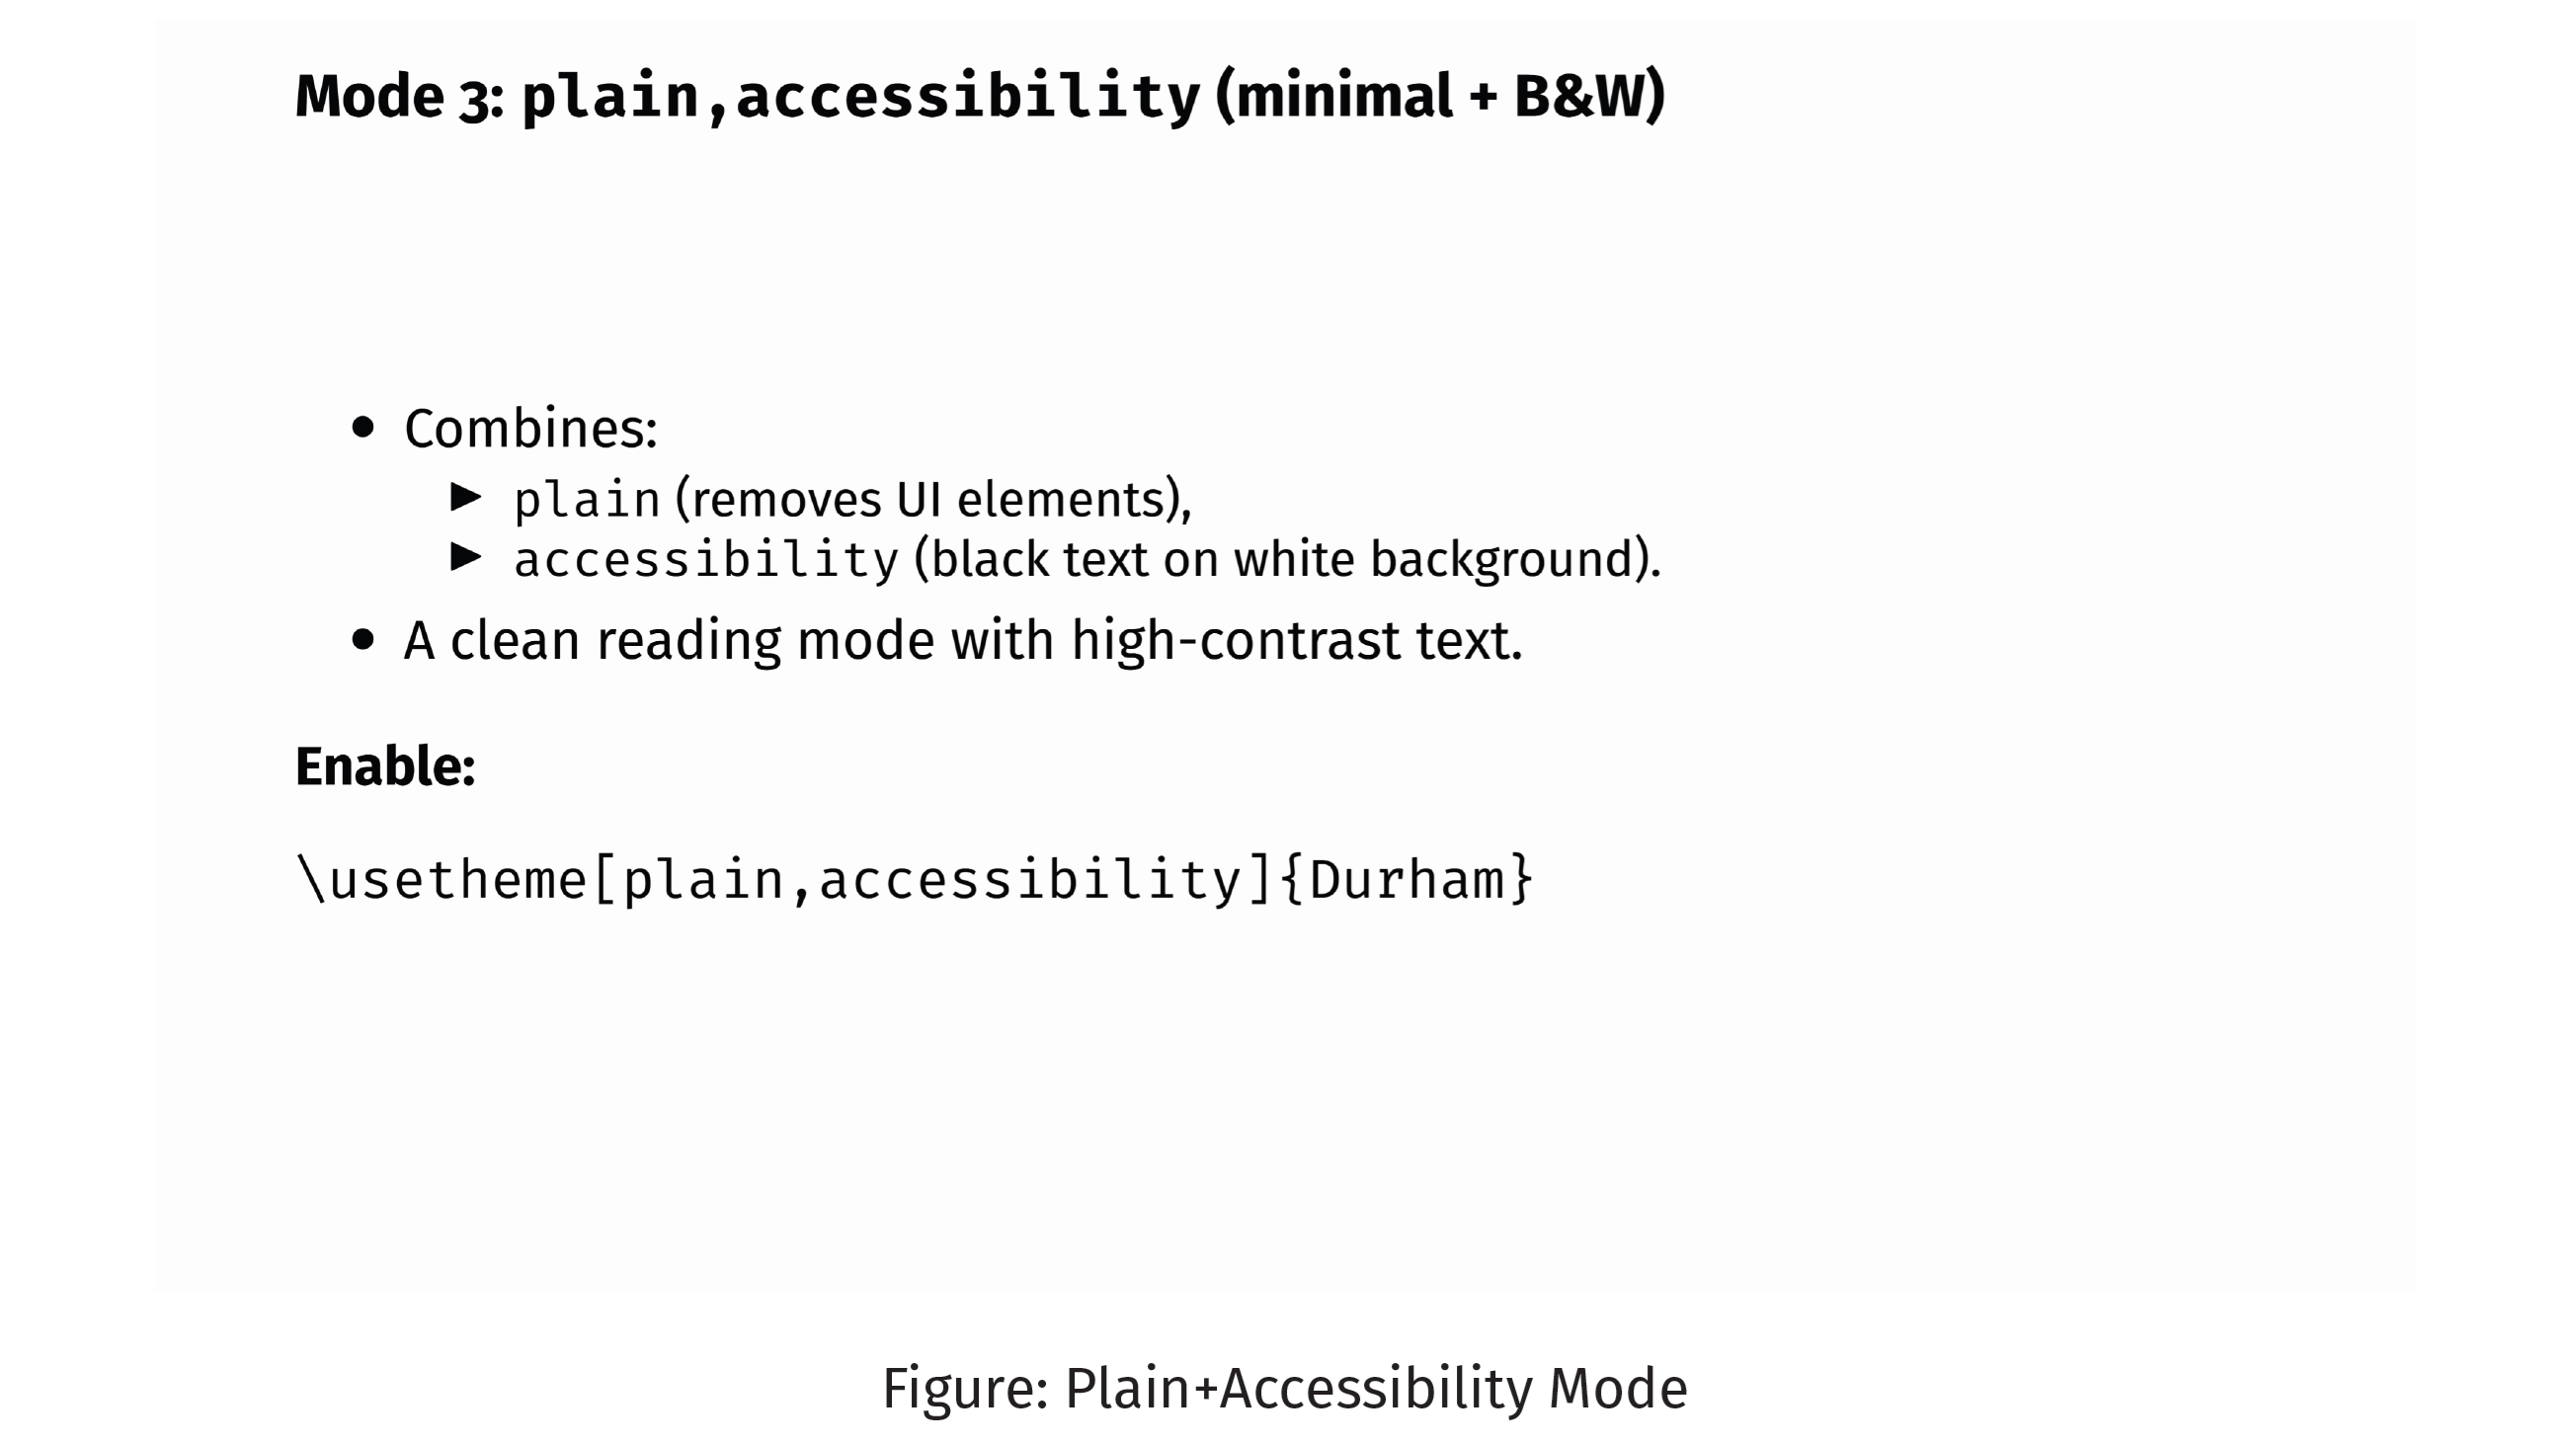
\includegraphics[width=1\linewidth]{plain_accessibility.png}
    \caption{Plain+Accessibility Mode}
\end{figure}
    
\end{frame}

\begin{frame}[fragile]{Mode 4: \texttt{plain,accessibility,invert} (minimal + dark)}
\begin{itemize}
  \item A dark reading mode for users uncomfortable with bright backgrounds.
  \item Combines:
  \begin{itemize}
    \item \texttt{plain}: removes headline/footline/progress,
    \item \texttt{accessibility}: enforces high contrast,
    \item \texttt{invert}: black background with white text.
  \end{itemize}
\end{itemize}

\vspace{0.8em}
\textbf{Enable:}
\begin{verbatim}
\usetheme[plain,accessibility,invert]{durham}
\end{verbatim}
\end{frame}

\begin{frame}[plain]
\begin{figure}
    \centering
    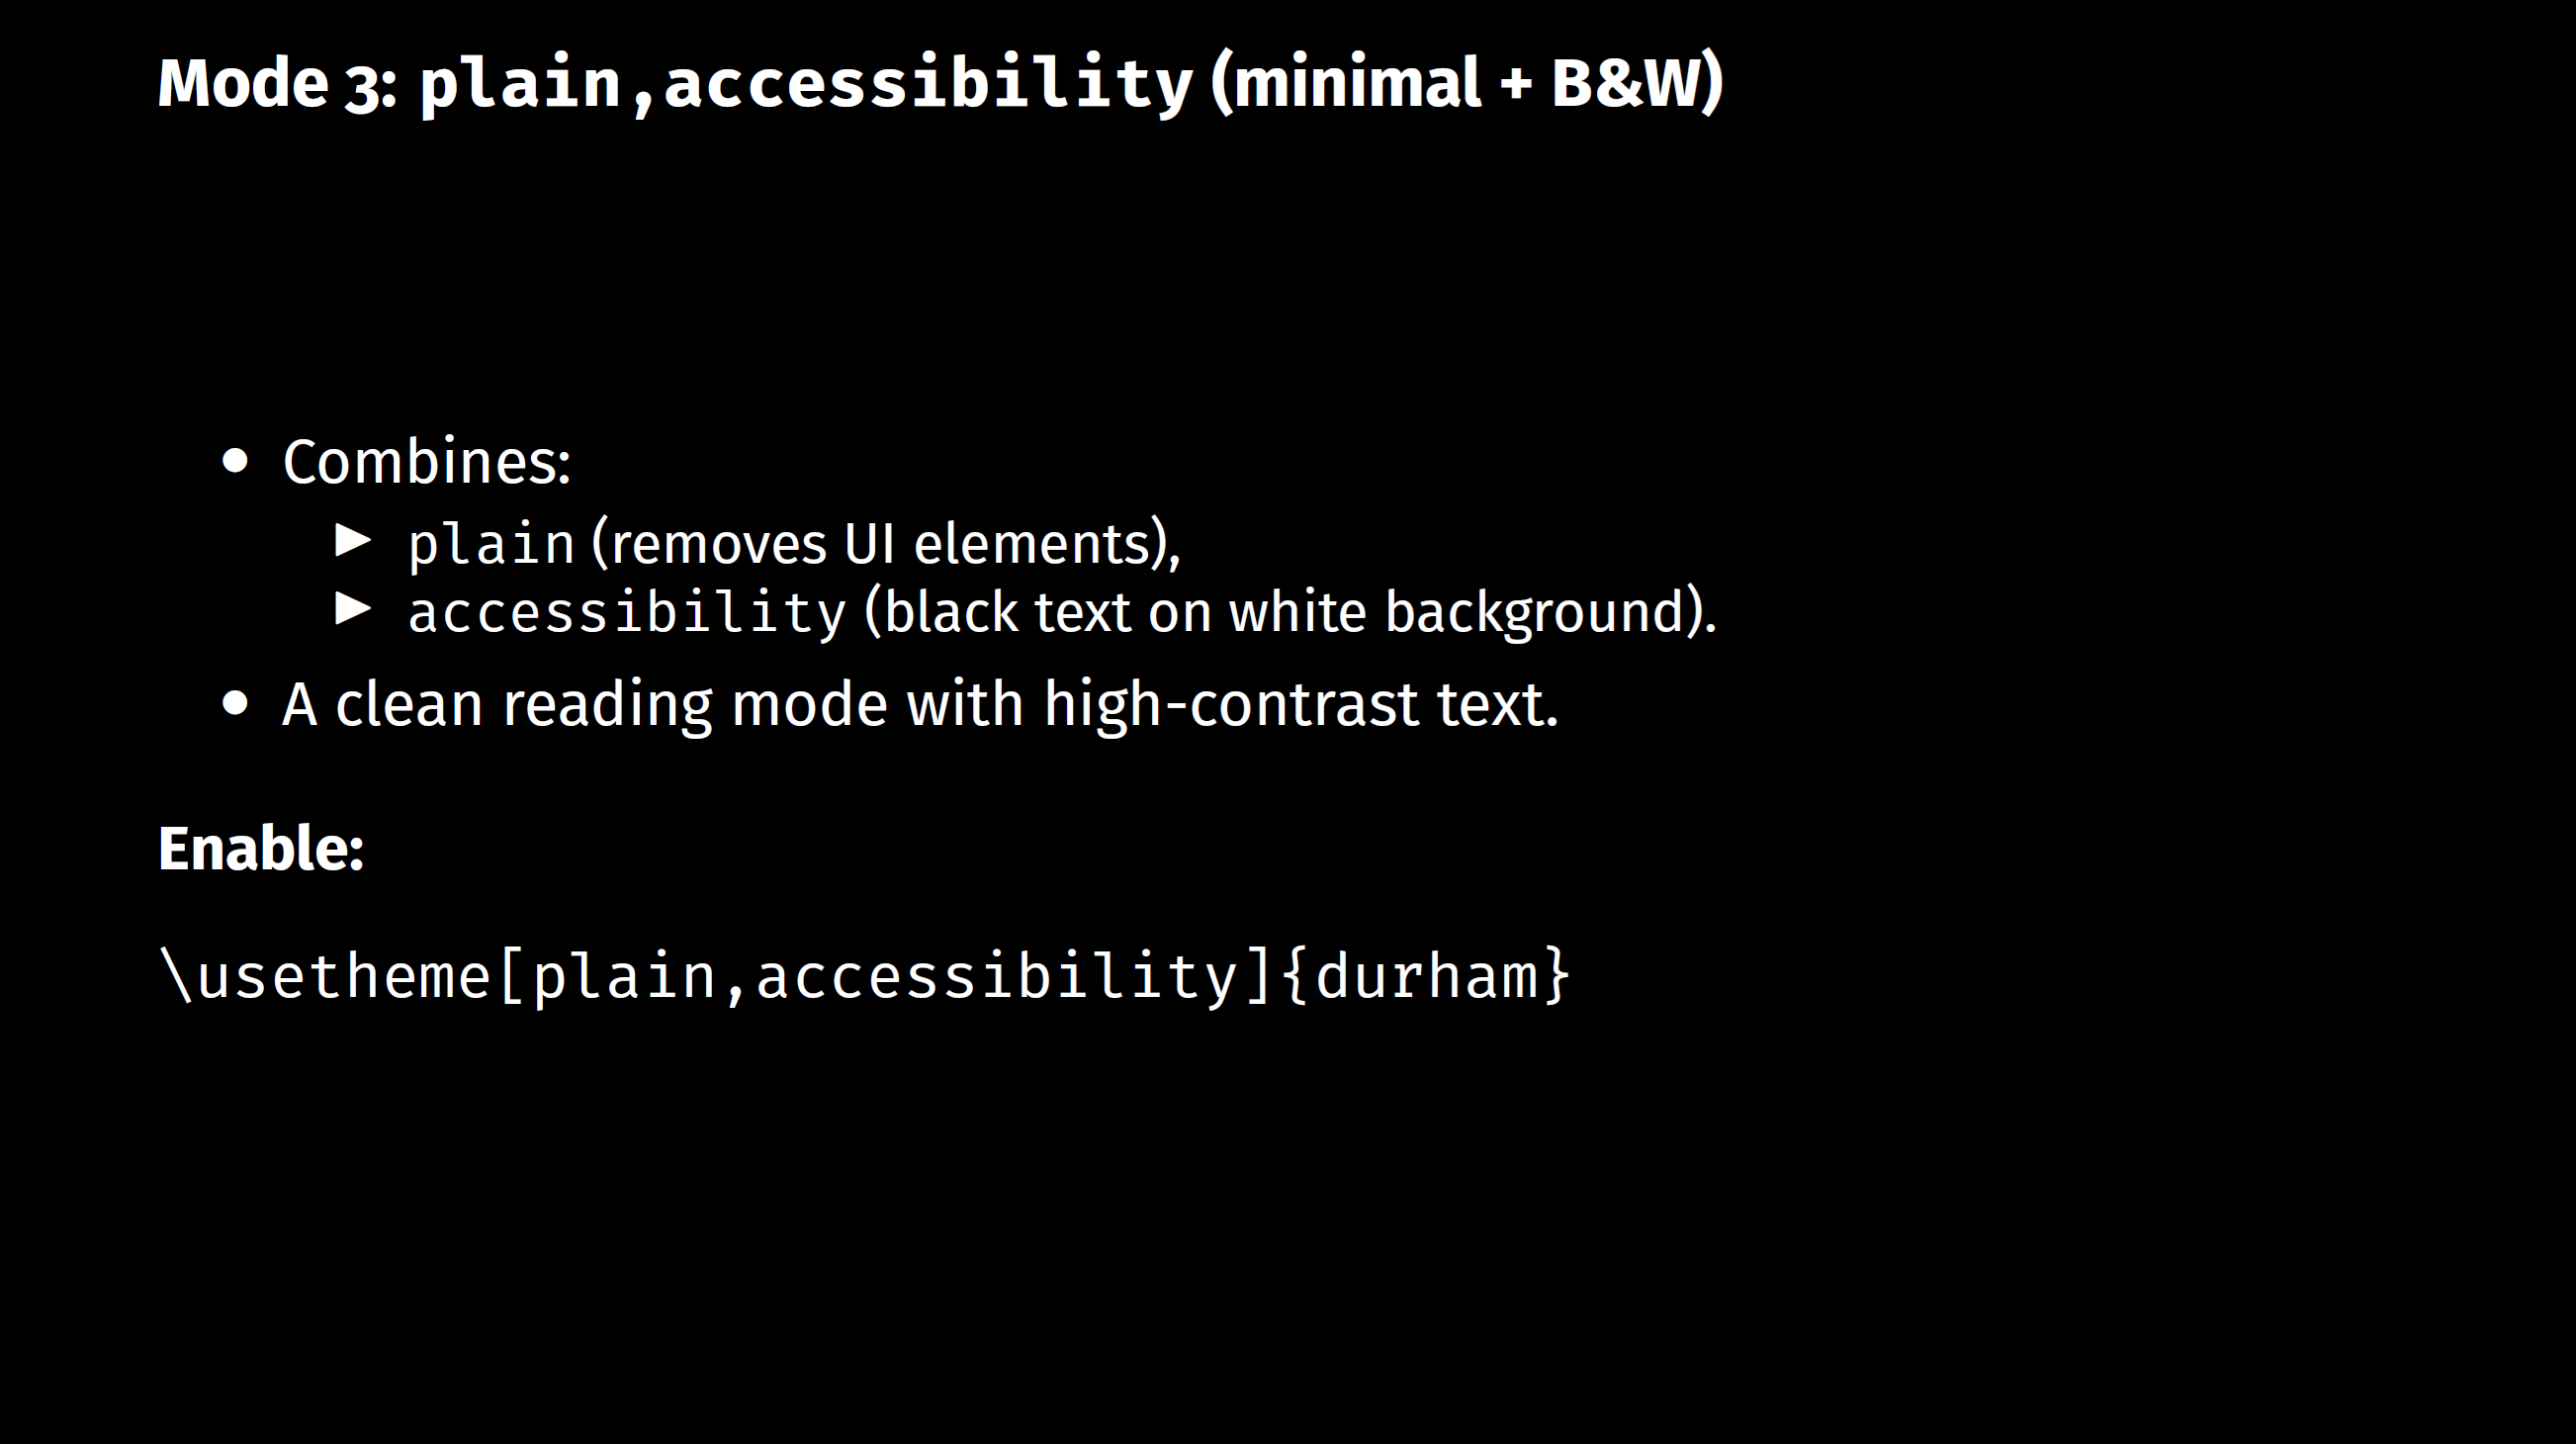
\includegraphics[width=1\linewidth]{plain_accessibility_invert.png}
    \caption{Plain+Accessibility+Invert Mode}
\end{figure}
\end{frame}

\begin{frame}{Accessibility note}
\begin{itemize}
  \item These options address \textbf{visual accessibility}:
  contrast, colour dependence, and reading comfort.
  \item For \textbf{screen readers / tagged PDF}, Beamer output can be limited by
  the current PDF tagging toolchain.
  \item Within these constraints, the theme addresses the aspects of accessibility that are realistically controllable at the theme level.
  \item Best practice (when required): provide an accessible companion output
  (e.g., detailed notes or a tagged handout) alongside slides.

\end{itemize}
\end{frame}


%========================================================
\section{Conclusion}
%========================================================

\begin{frame}{Content-first approach}
The Durham Beamer theme represents:
\begin{itemize}
  \item a shift from slide-centric to lecture-centric design,
  \item an explicit focus on pedagogy rather than aesthetics,
  \item a practical response to accessibility and inclusivity.
\end{itemize}
\end{frame}

\begin{frame}{Outcome and reflection}
Rather than offering a single visual style, the theme provides:
\begin{itemize}
  \item a coherent presentation system,
  \item adaptable modes for different teaching contexts,
  \item a structure that supports both lecturers and students.
\end{itemize}

\vspace{0.6em}
It demonstrates how careful design of presentation technology can support teaching practice.
\end{frame}

\begin{frame}{Closing thought}
Good teaching tools should:
\begin{itemize}
  \item stay out of the way of content,
  \item respect the diversity of learners,
  \item and support, rather than dictate, pedagogy.
\end{itemize}

\vspace{0.8em}
The Durham theme is a small but deliberate step in that direction.
\end{frame}

\makethankyou

\end{document}
